\documentclass[compress]{beamer}
\usepackage{ifthen,verbatim,ulem}

\title{Alignment Progress, Startup Alignment, and Comparison with Optical Alignment}
\author{Jim Pivarski, Alexei Safonov, K\'aroly Banicz$^*$}
\institute{Texas A\&M University, $^*$FermiLab}
\date{23 February, 2008}

\newcommand{\isnote}{}
\xdefinecolor{lightyellow}{rgb}{1.,1.,0.25}
\xdefinecolor{darkblue}{rgb}{0.1,0.1,0.7}

%% Uncomment this to get annotations
%% \def\notes{\addtocounter{page}{-1}
%%            \renewcommand{\isnote}{*}
%% 	   \beamertemplateshadingbackground{lightyellow}{white}
%%            \begin{frame}
%%            \frametitle{Notes for the previous page (page \insertpagenumber)}
%%            \itemize}
%% \def\endnotes{\enditemize
%% 	      \end{frame}
%%               \beamertemplateshadingbackground{white}{white}
%%               \renewcommand{\isnote}{}}

%% Uncomment this to not get annotations
\def\notes{\comment}
\def\endnotes{\endcomment}

\setbeamertemplate{navigation symbols}{}
\setbeamertemplate{headline}{\mbox{ } \hfill
\begin{minipage}{5.5 cm}
\vspace{-0.75 cm} \small
\end{minipage} \hfill
\begin{minipage}{4.5 cm}
\vspace{-0.75 cm} \small
\begin{flushright}
\ifthenelse{\equal{\insertpagenumber}{1}}{}{Jim Pivarski \hspace{0.2 cm} \insertpagenumber\isnote/\pageref{numpages}}
\end{flushright}
\end{minipage}\mbox{\hspace{0.2 cm}}\includegraphics[height=1 cm]{../cmslogo} \hspace{0.1 cm} \includegraphics[height=1 cm]{../tamulogo} \hspace{0.01 cm} \vspace{-1.05 cm}}

\begin{document}
\frame{\titlepage}

%% \begin{notes}
%% \item This is the annotated version of my talk.
%% \item If you want the version that I am presenting, download the one
%% labeled ``slides'' on Indico (or just ignore these yellow pages).
%% \item The annotated version is provided for extra detail and a written
%% record of comments that I intend to make orally.
%% \item Yellow notes refer to the content on the {\it previous} page.
%% \item All other slides are identical for the two versions.
%% \end{notes}

\begin{frame}
\frametitle{Alignment needs}

\begin{itemize}\setlength{\itemsep}{0.4 cm}
\item for analysis:
\begin{itemize}\setlength{\itemsep}{0.1 cm}
\item Procedure for aligning with large datasets (10/100~pb$^{-1}$)
\item All the necessary software tools
\item Full systematics studies
\end{itemize}

\item for commissioning:
\begin{itemize}\setlength{\itemsep}{0.1 cm}
\item Procedure that uses minimal collisions data
\item Tests with real data
\item Procedures for integration with optical alignment
\end{itemize}

\item for validation:
\begin{itemize}\setlength{\itemsep}{0.1 cm}
\item Monitoring plots
\item Comparison with optical alignment
\end{itemize}
\end{itemize}
\end{frame}

\begin{frame}
\frametitle{Long-term alignment procedure}
\begin{itemize}\setlength{\itemsep}{0.4 cm}
\item Baseline procedure is stable and has been for some time
\begin{itemize}\setlength{\itemsep}{0.15 cm}
\item Based on the HIP algorithm
\item Aligns one station at a time (from the inside out)
\end{itemize}
\item Hierarchial structure of the code matches system design
\begin{itemize}\setlength{\itemsep}{0.15 cm}
\item Fast alignment of large structures ($\sim$1000 muons)
\item Built-in support for constraints from prior knowledge,
photogrammetry, optical system
\item Possible to combine measurements from different sources
\end{itemize}
\item Optimization of parameters is in progress for faster convergence
and better accuracy
\begin{itemize}\setlength{\itemsep}{0.15 cm}
\item Track-fitting parameters (APEs) tuned for each station
\item Intelligent track selection to supress strongly scattering tracks
\item Optimized track-fitting to better use structure of the detector
and material distribution (pending tests)
\end{itemize}
\end{itemize}
\end{frame}

\begin{frame}
\frametitle{Long-term alignment procedure}

100~pb$^{-1}$ simulation results

Illustration of improvements (``intelligent track selection'')

\vspace{-0.5 cm}
\begin{center}
\begin{tabular}{p{0.45\linewidth} p{0.45\linewidth}}
\begin{center}Baseline procedure\end{center} & \begin{center}Test of track-cut\end{center}
\end{tabular}

\vspace{-0.5 cm}
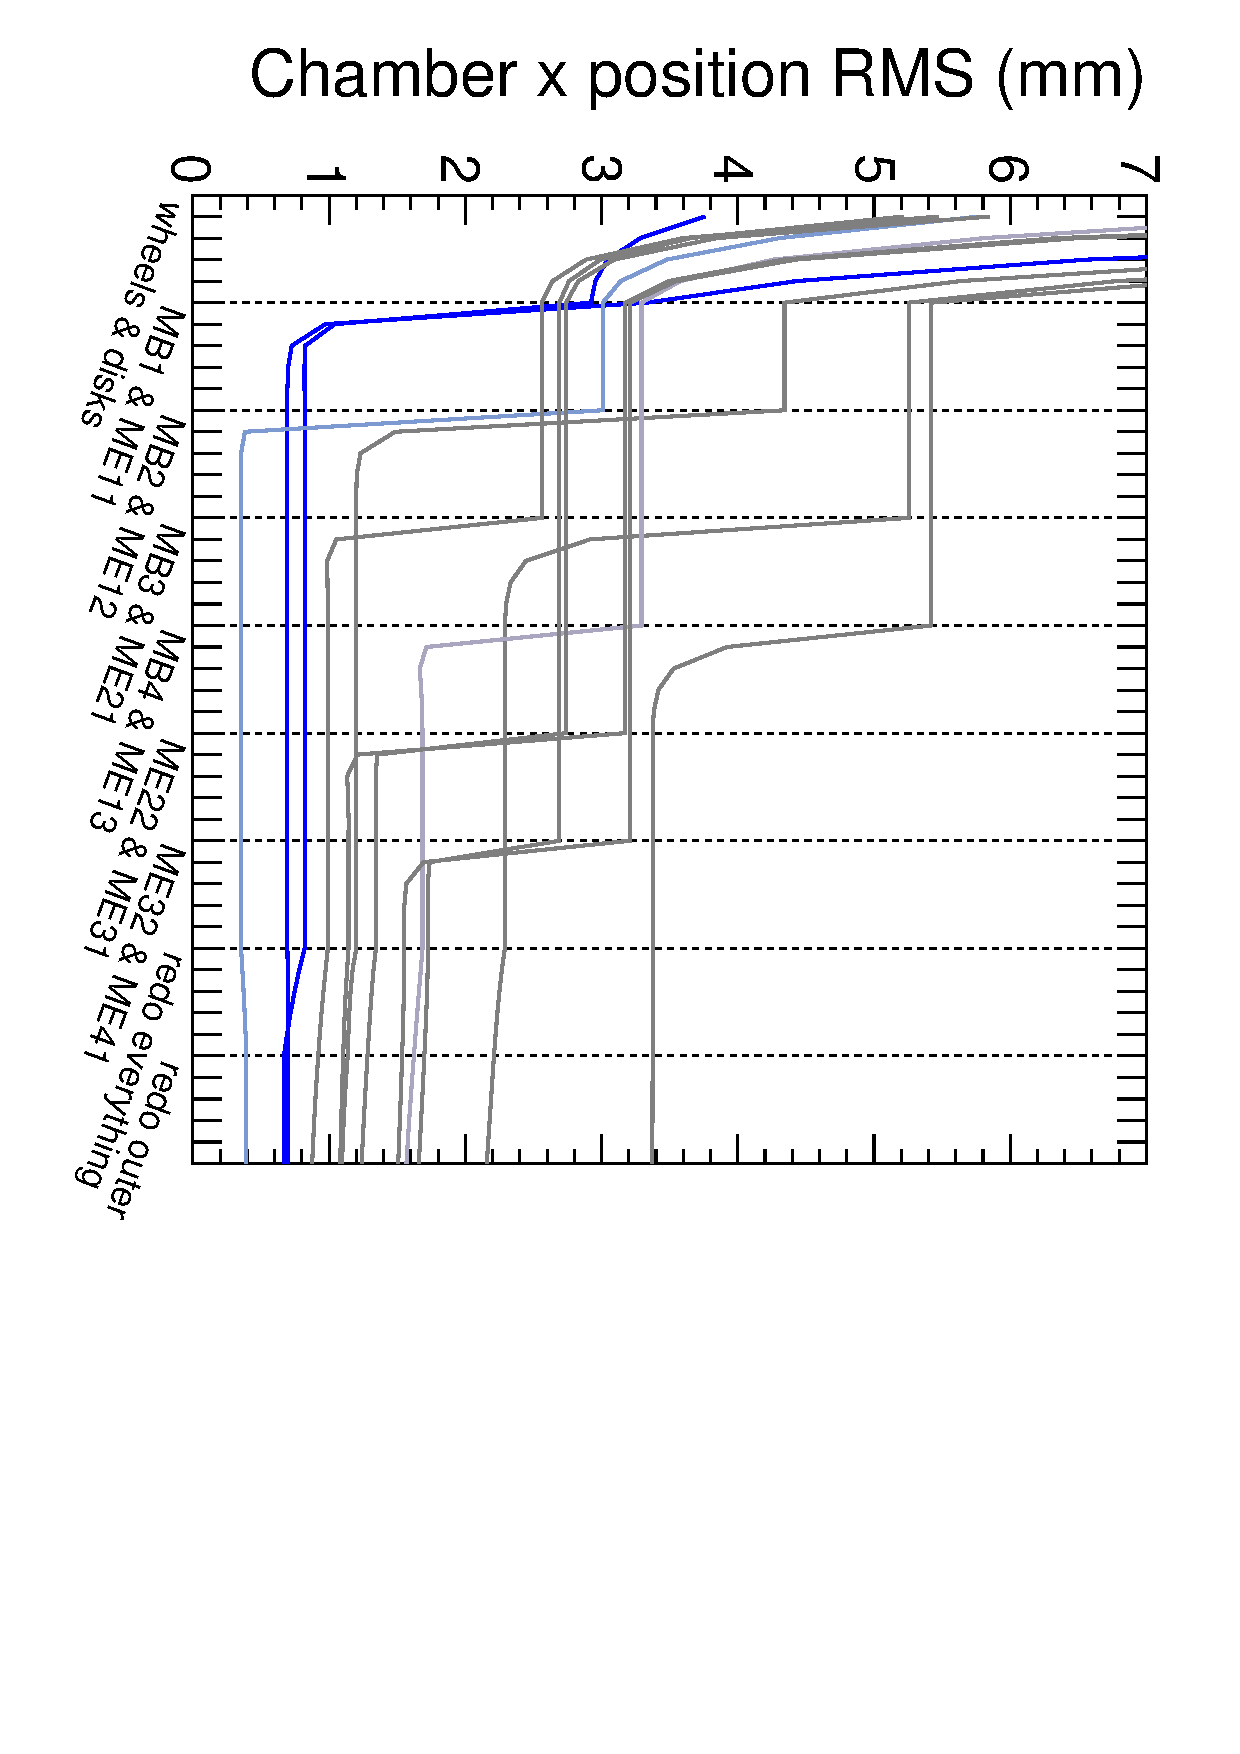
\includegraphics[width=5. cm, angle=90]{convergence-100.pdf}
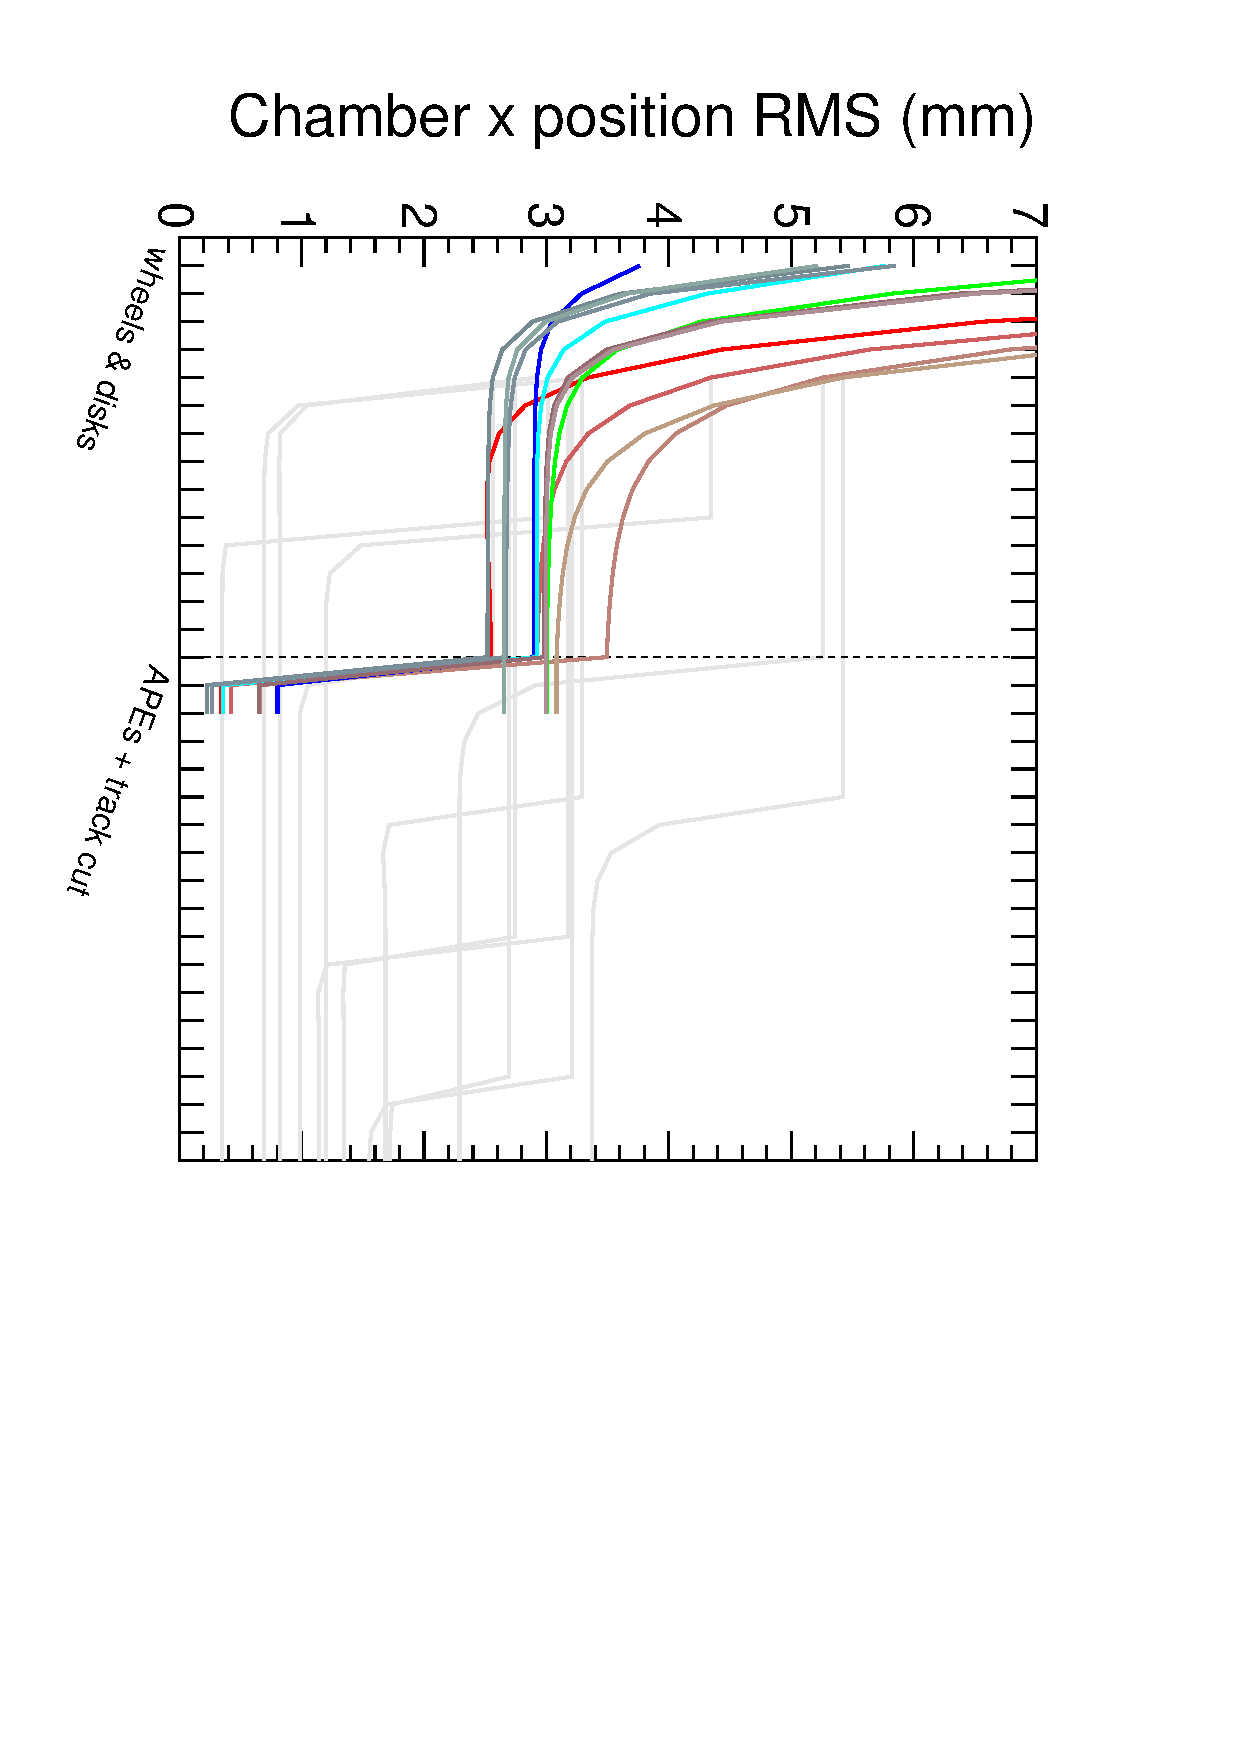
\includegraphics[width=5. cm, angle=90]{large_APEs_trackcut-100.pdf}
\end{center}

Each line is a station's resolution as a function of iteration

Improved alignment reaches 300~$\mu$m for inner stations (which drive momentum resolution)
\end{frame}

\begin{frame}
\frametitle{Commissioning \& early alignment}
\hspace{-0.83 cm} \textcolor{darkblue}{\Large become primary focus (and subject for this talk)}

\begin{itemize}
\item Can't accurately align all chambers with limited statistics
\item But can quickly align large structures if internal alignment is known from other sources
\item Track-based candidates:
\begin{itemize}
\item beam-halo perfect for endcap
\item cosmics for barrel
\end{itemize}
\item Optical very useful for cross-checks and filling in gaps
\begin{itemize}
\item e.g.\ $z$ alignment, to which beam-halo is insensitive
\end{itemize}
\end{itemize}

\hspace{-0.83 cm} \textcolor{darkblue}{\Large Outline}
\begin{enumerate}
\item Procedures for endcap alignment without \mbox{any (many) collisions\hspace{-1 cm}}
\item How to test these procedures with cosmic rays
\item Procedures and tools for comparison and integration with optical alignment
\item Status of software tools
\end{enumerate}
\end{frame}

\begin{frame}
\frametitle{Motivation...}

Momentum resolution depends on absolute alignments, which are a combination of
\[ \sigma_{\mbox{absolute}} = \sqrt{{\sigma_{\mbox{relative chambers}}}^2 + {\sigma_{\mbox{ring}}}^2} \]

\begin{center}
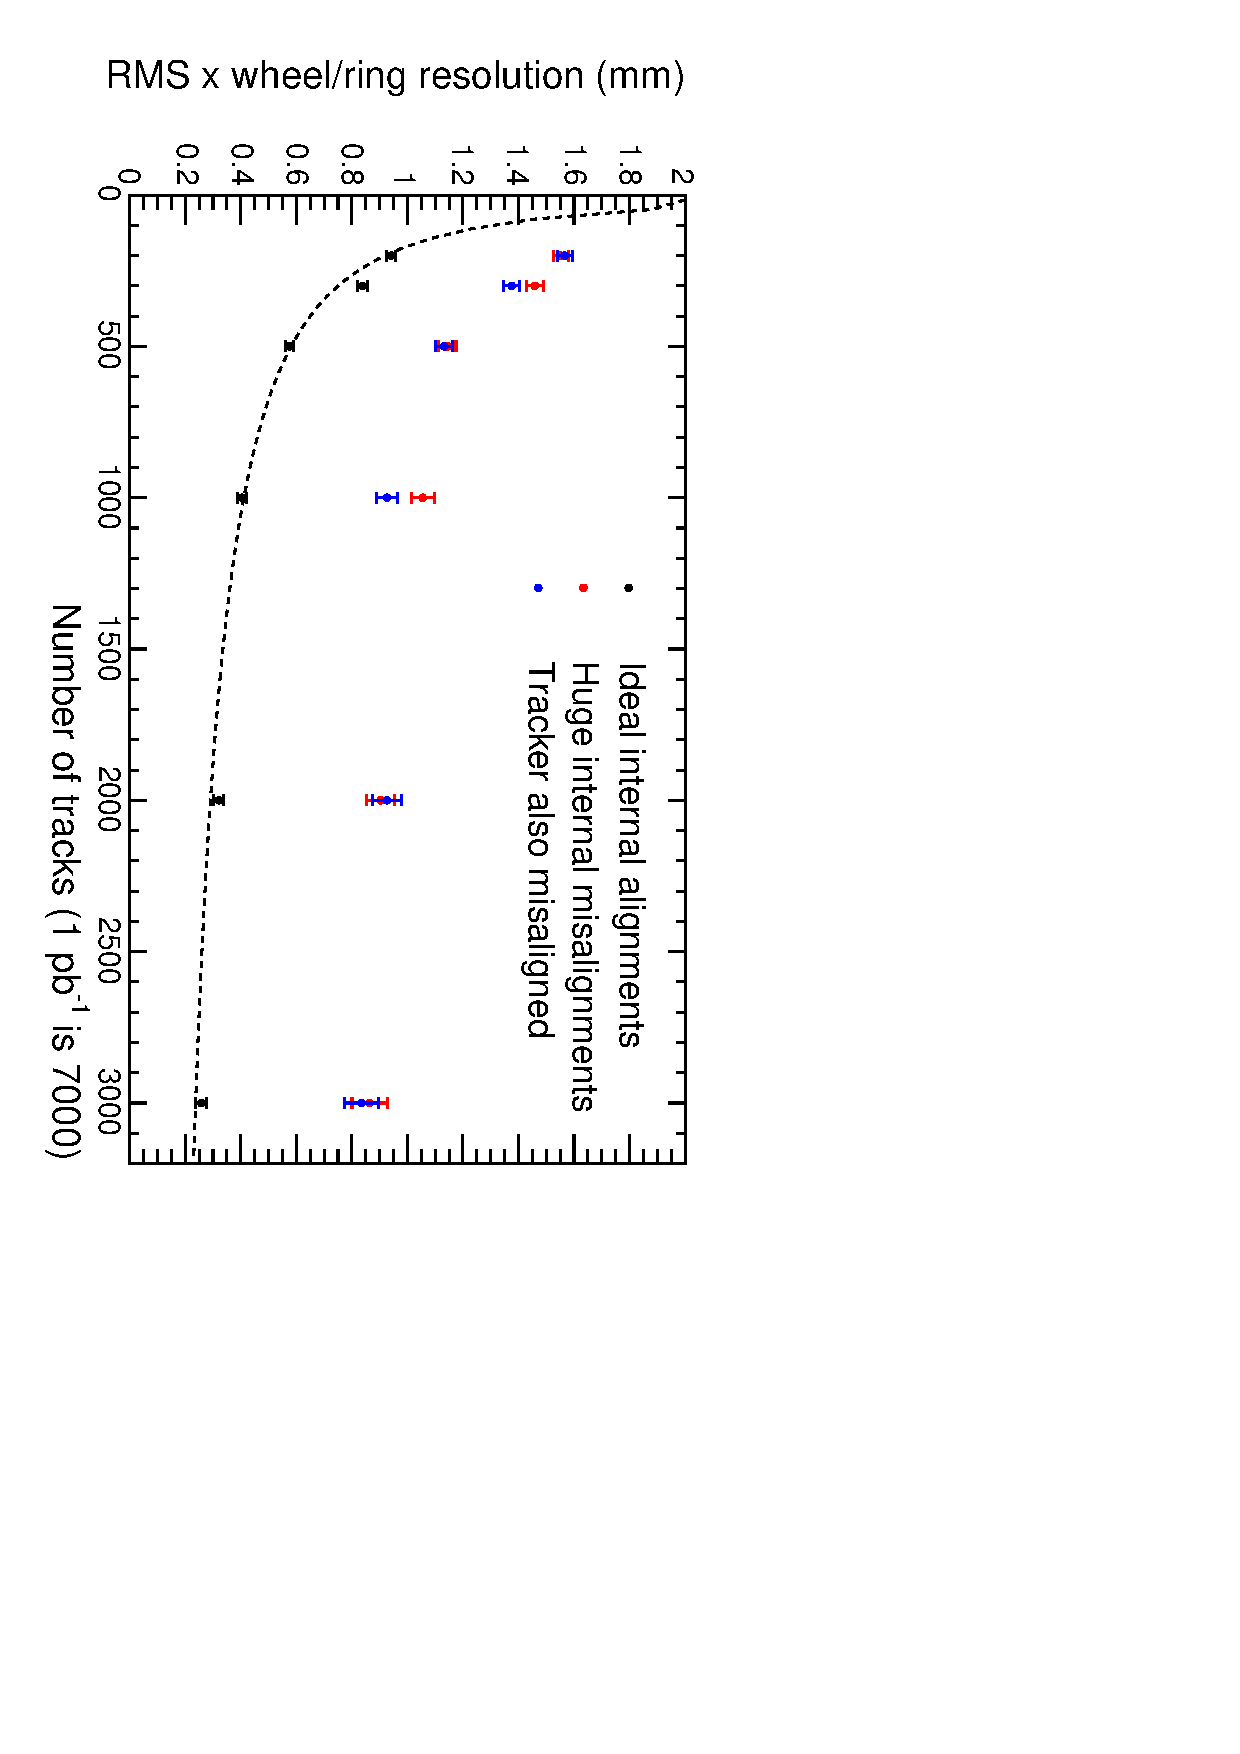
\includegraphics[height=0.9\linewidth, angle=90]{vsntracks.pdf}
\end{center}

With well-aligned chambers in a ring, we can very quickly establish full absolute alignment
\end{frame}

\begin{frame}
\frametitle{Wheel/ring simulation results}
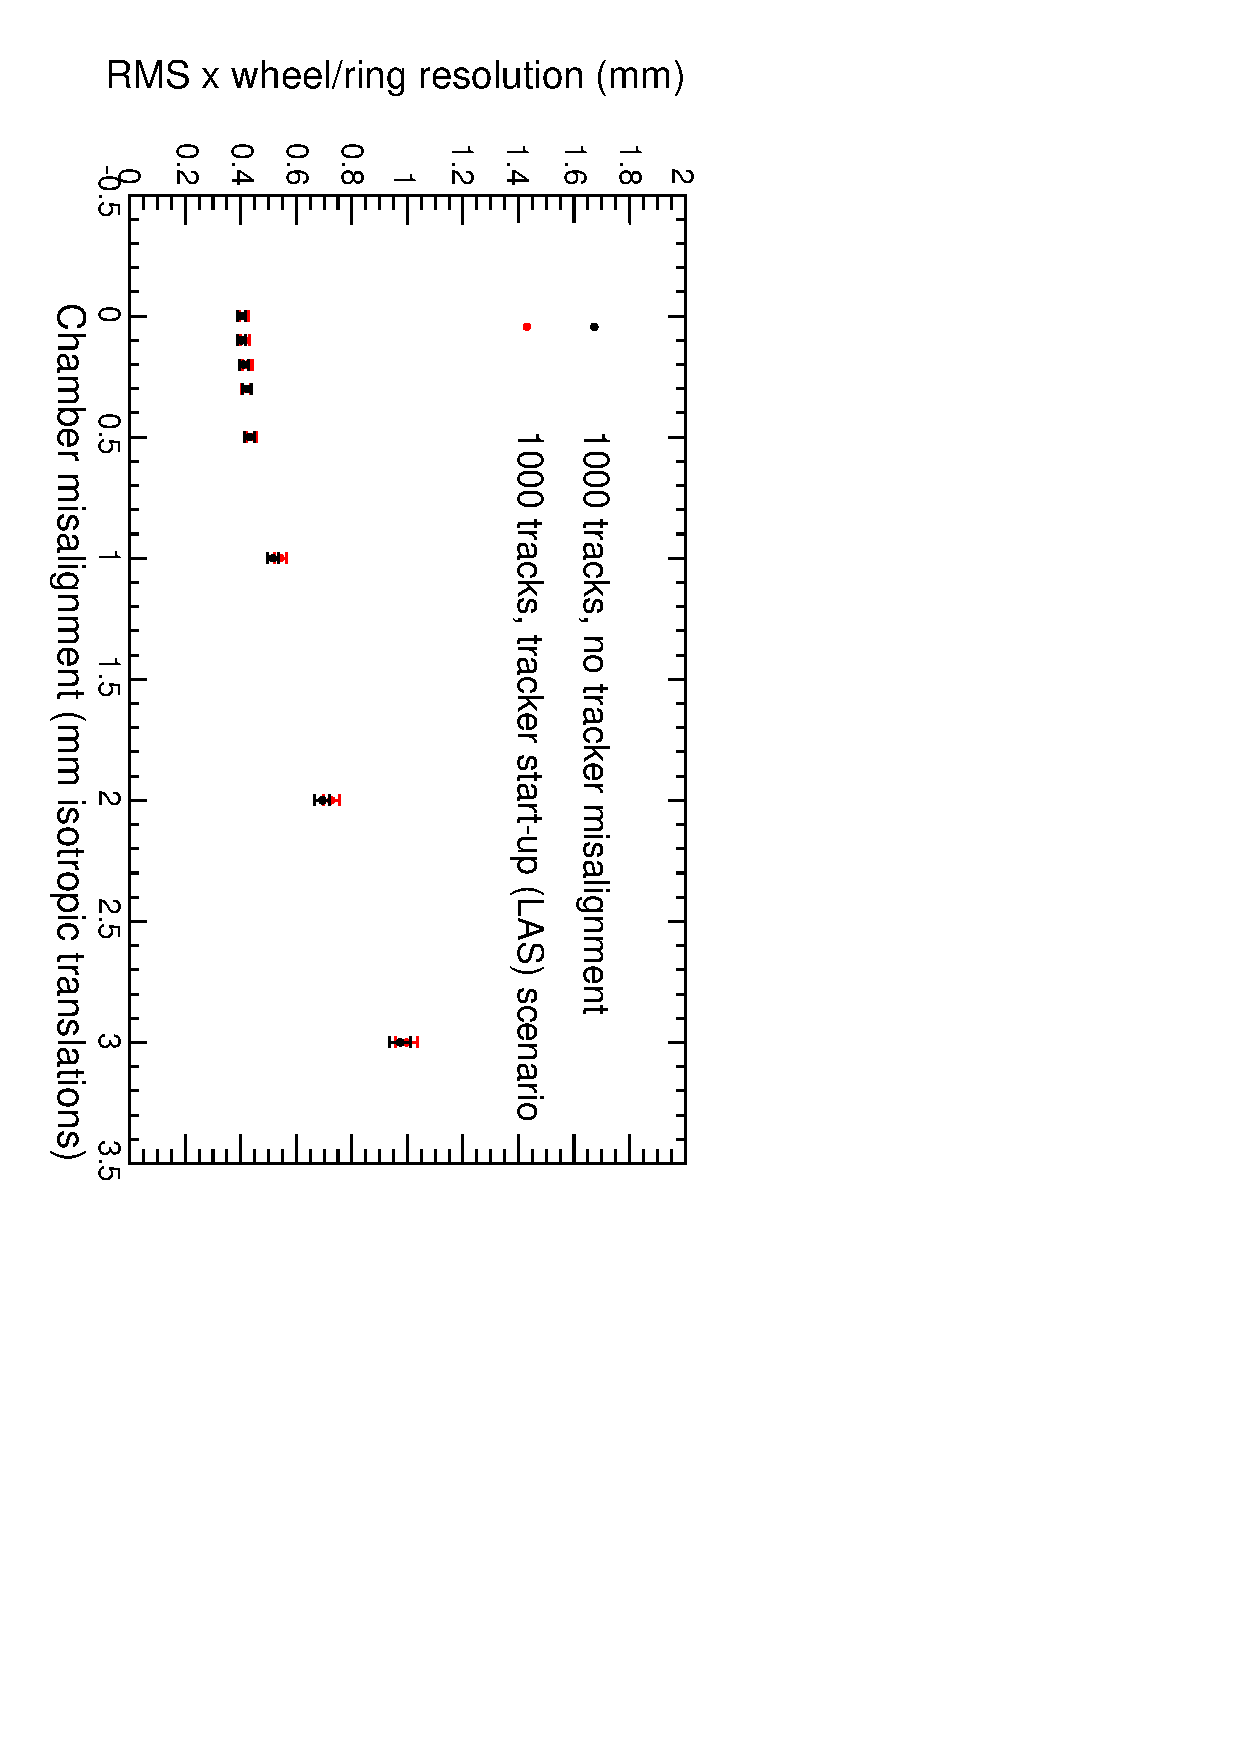
\includegraphics[height=\linewidth, angle=90]{vsinternal.pdf}
\begin{itemize}
\item With $\sim$1~mm chamber misalignments, $x$-$y$ 0.6~mm, $z$ 3~mm, $\phi_z$ 0.1~mrad
\item Tracker misalignment is negligible for such large solid angles
\end{itemize}
\end{frame}




\begin{frame}
\frametitle{No collisions alignment}

\vspace{-0.2 cm}
\begin{columns}
\column{0.8\linewidth}
\begin{itemize}\setlength{\itemsep}{0.2 cm}
\item Beam-halo through overlap regions (no ME1/3)
\item Minimal track propagation, measure $x$, $y$, \textcolor{gray}{$\phi_y$,} $\phi_z$
\item Beam-halo rate hard to predict
\item With sufficient rate, good for layer alignment
\item Chambers are aligned relative to one another within each ring
\end{itemize}
\column{0.2\linewidth}
\mbox{ }
\vspace{1 cm}

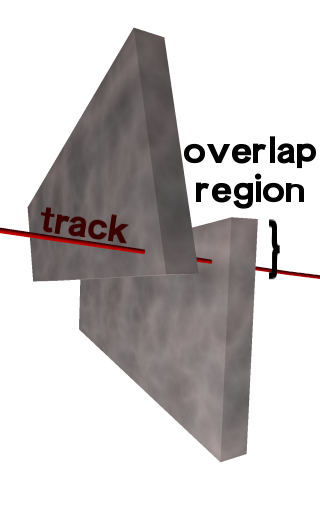
\includegraphics[width=\linewidth]{overlap.png}
\end{columns}

\hspace{-0.83 cm} \textcolor{darkblue}{\Large Few-collisions alignment}

\vspace{0.1 cm}
\begin{itemize}\setlength{\itemsep}{0.2 cm}
\item Align rings relative to tracker with 1000 GlobalMuons
\item Compliments beam-halo for a complete alignment
\end{itemize}

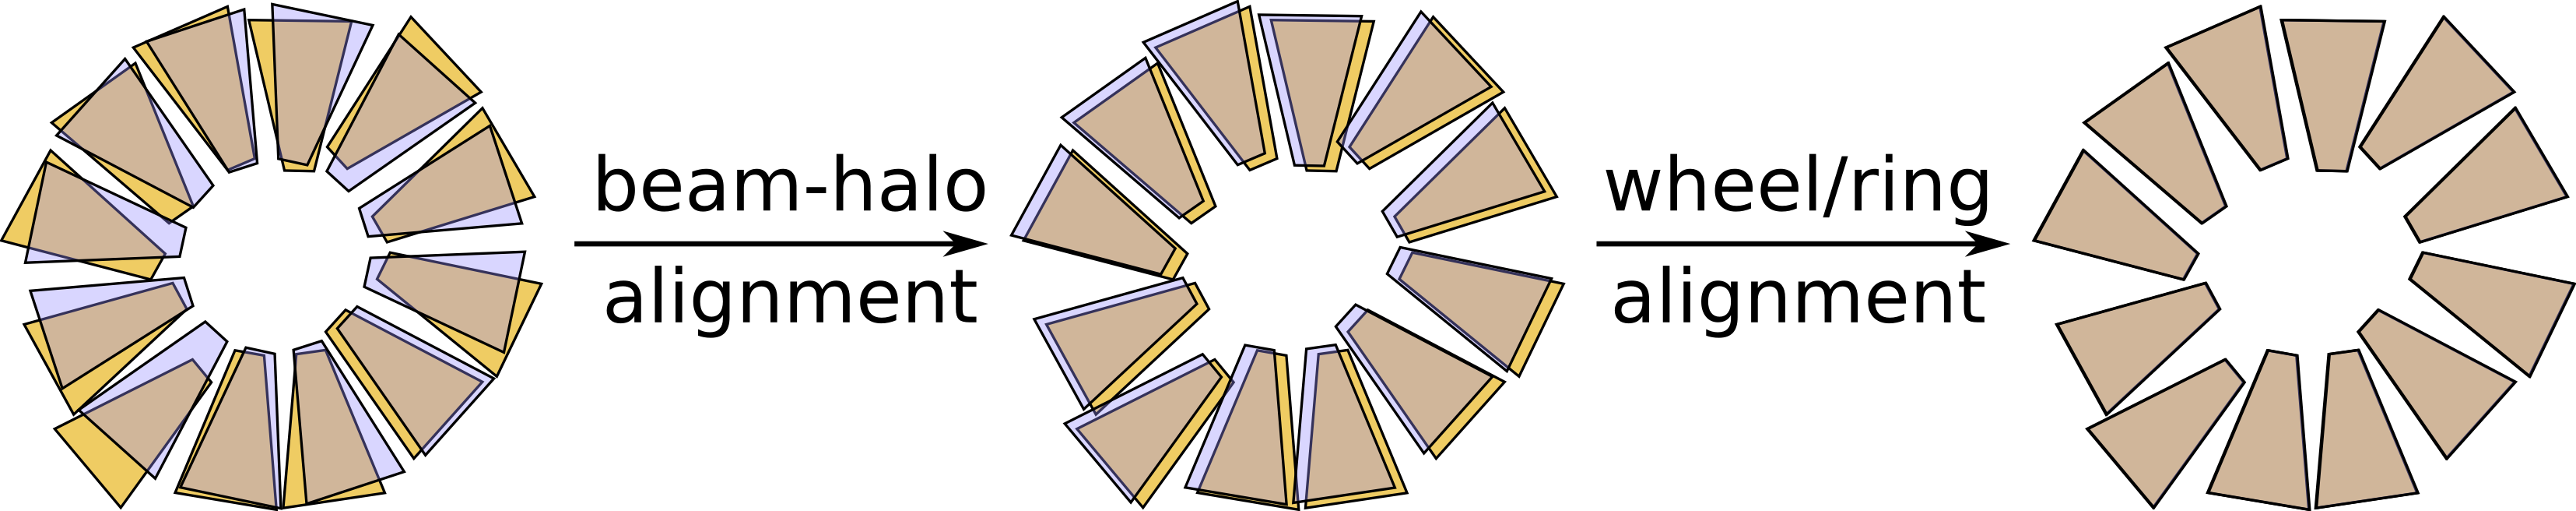
\includegraphics[width=\linewidth]{two_step_procedure.png}
\end{frame}

\begin{frame}
\frametitle{Beam-halo: K\'aroly Banicz}
\begin{itemize}
\item 6600 tracks/sec $\times$ 0.02 in overlap = 130~Hz~
\includegraphics[height=0.55\baselineskip]{timesdiv.png}100
\item 2~hours $\times$ 130~Hz = 1~million muons $\to$ \mbox{100's~of~$\mu$m~resolution~\hspace{-2 cm}}

(if we're off by $\times$100, 2~hours $\to$ 8 days\ldots)
\item Steeply falling function of energy and radius (better for ring 1)
\end{itemize}

\begin{center}
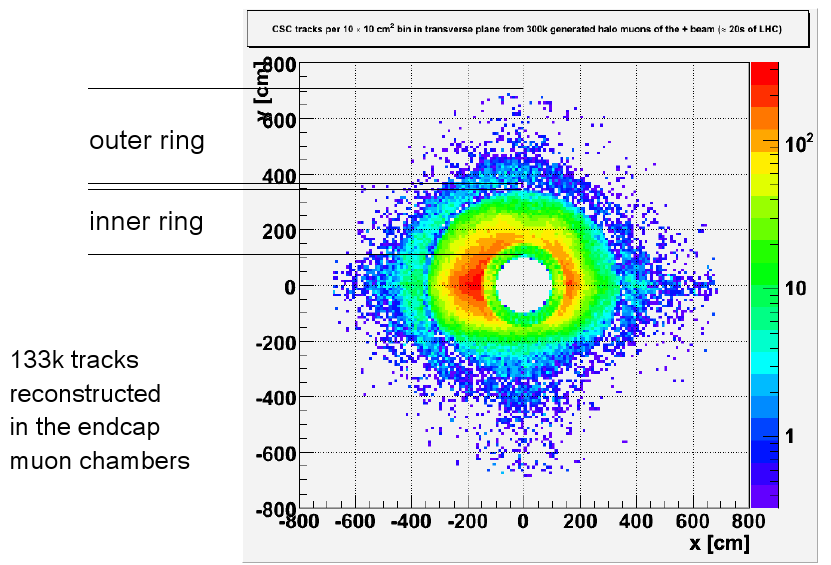
\includegraphics[width=0.8\linewidth]{beam-halo.png}
\end{center}
\end{frame}

\begin{frame}
\frametitle{Beam-halo procedure}
\begin{itemize}
\item Uses the same framework, reconfigured for local alignments
\item Tightly refit tracks to even-numbered chambers in a station,
loosely fit to odd-numbered to get local extrapolation from even to
odd
\item Alternate and repeat
\end{itemize}

\begin{center}
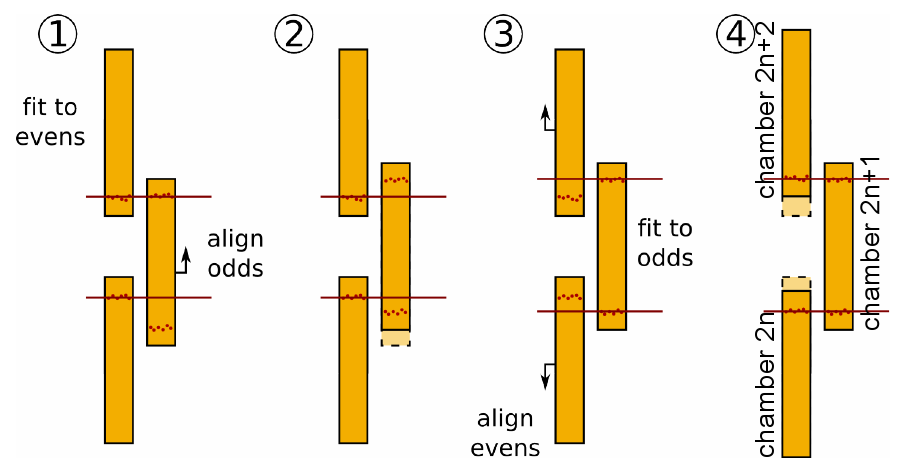
\includegraphics[width=0.87\linewidth]{even-odd.png}
\end{center}

\vspace{-0.25 cm}
\begin{itemize}
\item Repeat process with layers when enough tracks are available
\end{itemize}
\end{frame}




\begin{frame}
\frametitle{Early alignment timescales}
\begin{itemize}\setlength{\itemsep}{0.4 cm}
\item Beam-halo
\begin{itemize}\setlength{\itemsep}{0.1 cm}
\item Beginning with single-beam in June
\item Rate estimates are high but uncertain: na\"ive \mbox{worst~case~$\sim$8~days\hspace{-1 cm}}
\item Continue to collect beam-halo during normal data-taking
\end{itemize}

\item Start-up wheel/ring
\begin{itemize}
\item Beginning with first collisions in July(?)
\item $\le$ 4 days
\end{itemize}
\end{itemize}
\begin{center}
\small ``First month'' integrated luminosity ramp-up

\vspace{0.1 cm}
\renewcommand{\arraystretch}{1.1}
\begin{tabular}{c c c}
Bunches & Luminosity (cm$^{-2}$/s) & Time for 1000 muons ($W$, $Z$) \\\hline
1 $\times$ 1 & $10^{27}$ & \sout{\hspace{0.5 cm}4.1 years\hspace{0.5 cm}} \\
43 $\times$ 43 & $3.8 \times 10^{29}$ & 4.0 days \\
43 $\times$ 43 & $1.7 \times 10^{30}$ & 21 hours \\
43 $\times$ 43 & $6.1 \times 10^{30}$ & 5.9 hours \\
156 $\times$ 156 & $1.1 \times 10^{31}$ & 3.3 hours \\
156 $\times$ 156 & $5.6 \times 10^{31}$ & 39 minutes \\
156 $\times$ 156 & $1.1 \times 10^{32}$ & 20 minutes \\
\end{tabular}
\end{center}
\end{frame}

\begin{frame}
\frametitle{Testing with data before June}

\textcolor{darkblue}{Beam-halo procedure}
\begin{itemize}\setlength{\itemsep}{0.1 cm}
\item Run beam-halo procedure on horizontal MTCC cosmic rays
\end{itemize}

\vfill
\textcolor{darkblue}{GlobalMuon procedures (wheel/ring and chamber-level)}
\begin{itemize}\setlength{\itemsep}{0.1 cm}
\item April CRAFT cosmic ray run includes full tracker
\item Select near-IP muons: $\sim$1 million through barrel wheel 0

$\sim$10,000 in ME1/3 (which has no overlap hits for beam-halo)
\end{itemize}

\vfill
Need beam-halo, cosmic ray MC, MTCC reprocessed in 2\_0\_0,

HLT paths and AlCa streams for real beam-halo and cosmic rays
\end{frame}

\begin{frame}
\frametitle{Optical comparisons: 0~pb$^{-1}$}

\begin{columns}
\column{0.8\linewidth}
\begin{itemize}\setlength{\itemsep}{0.2 cm}
\item Beam-halo and SLM lines both measure $x$
\item SLM lines can also measure $z$
\item Caveats
\begin{itemize}
\item Beam-halo and optical must both work in the same ring coordinates
\item Track-based measures strips and wires, \\ optical measures the box: must know layer positions relative to alignment pins
\end{itemize}
\end{itemize}
\column{0.2\linewidth}
\mbox{ }
\vspace{1 cm}

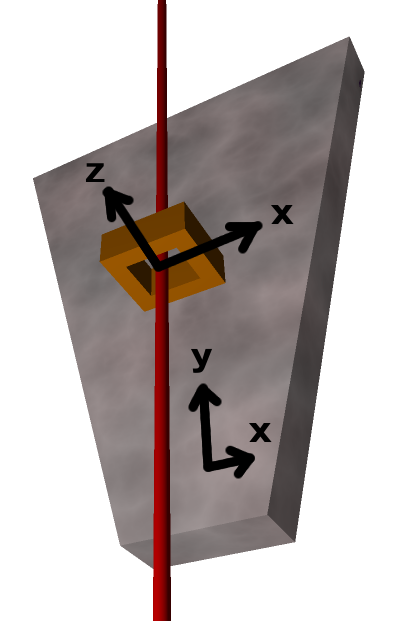
\includegraphics[width=\linewidth]{comparison/comparison.png}
\end{columns}

\vfill
\textcolor{darkblue}{Suggested procedure:}
\begin{enumerate}
\item Measure SLM lines underground at 4T, full COCOA fit
\item Propagate to averaged layer position through \mbox{layer~measurements\hspace{-1 cm}}
\item Constrain track-based ring positions to be the \mbox{same as COCOA\hspace{-1 cm}}
\item Align chambers within rings with beam-halo, compare $x$
\item If it agrees, apply $z$ measurement to ring ($z$, $\phi_x$, and $\phi_y$)
\end{enumerate}
\end{frame}

\begin{frame}
\vfill
\vfill
\vfill
\hspace{-0.83 cm} \textcolor{darkblue}{\Large Optical measurements: 1000 muons}

\begin{itemize}
\item Transfer lines, Z sensors measure outer ring in 6 d.o.f.
\item So does GlobalMuon alignment
\item GlobalMuon alignment puts rings into tracker coordinates
\item Tests full link system down to tracker in 6 d.o.f.
\end{itemize}

\vfill
\hspace{-0.83 cm} \textcolor{darkblue}{\Large Relevant measurements for comparison}

\begin{itemize}
\item MTCC SLM measurements for beam-halo MTCC test \hfill \textcolor{red}{$\surd$}
\item Barrel measurements during CRAFT GlobalMuon test in April
\item SLM measurements during beam-halo data-taking in June
\item Transfer line, Z sensor, link system measurements during start-up collisions in July
\item Integration of layer positions with SLM measurements
\item Output in CSCSurveyRcd format (to apply ring constraints)
\end{itemize}
\end{frame}

\begin{frame}
\frametitle{Software status}
\begin{itemize}
\item Parallelized 10/100~pb$^{-1}$ procedure \hfill \textcolor{red}{$\surd$}
\item Added CSCRing as an alignable structure \hfill \textcolor{red}{$\surd$}
\item DB $\leftrightarrow$ human-editable files and plots (monitoring) \hfill \textcolor{red}{$\frac{1}{2}$ done}
\item Tool for setting arbitary patterns of hit weights (APEs) \hfill \textcolor{red}{$\surd$}
\item Improved track cut and alternate refitter for upcoming tests \hfill \textcolor{red}{$\surd$}
\item Mechanism for setting global coordinate system \hfill \textcolor{red}{$\surd$}
\item HLT paths and AlCa streams for beam-halo, cosmics
\item Beam-halo and cosmic MC production cfg
\end{itemize}

\hspace{-0.83 cm} \textcolor{darkblue}{\Large Procedure status}
\begin{itemize}
\item 10/100~pb$^{-1}$ GlobalMuons: baseline working, can be optimized further, studied in more detail
\item Cosmic ray version of high-lumi GlobalMuons: need MC
\item Beam-halo: procedure designed, needs to be implemented
\item 1000 muon ring alignment: easy adaptation of GlobalMuon
\end{itemize}

\end{frame}

\begin{frame}
\frametitle{Conclusions}
\begin{itemize}\setlength{\itemsep}{0.4 cm}
\item Several different projects in parallel
\begin{itemize}\setlength{\itemsep}{0.15 cm}
\item Big alignments: relevant for physics reach
\item Little alignments: initial geometry without many collisions
\item Comparisons with optical: for commissioning, validation, dependence on time
\end{itemize}

\item All alignments tested in cosmic rays before any LHC beam (even single-beam)

\item Special alignment datasets need to be collected: \\ Making sure the data paths exist

\item Making sure all the software is written and submitted on time
\end{itemize}
\label{numpages}
\end{frame}

\begin{frame}
\frametitle{Suggested alignment scenarios}

\mbox{\hspace{-0.75 cm} \begin{tabular}{p{0.5 cm} c c c c c c}
\mbox{0~pb$^{-1}$ \textcolor{blue}{beam-halo} plus \textcolor{red}{optical} \hspace{-3 cm}} & & & & & & \\
& $x$ & $y$ & $z$ & $\phi_x$ & $\phi_y$ & $\phi_z$ \\
C & \textcolor{blue}{700~$\mu$m} & \textcolor{blue}{2~mm} & 3~mm & 3~mrad & \textcolor{blue}{0.8~mrad} & \textcolor{blue}{0.65~mrad} \\
R & \textcolor{red}{200~$\mu$m} & \textcolor{red}{200~$\mu$m} & \textcolor{red}{230~$\mu$m} & \textcolor{red}{0.08~mrad} & \textcolor{red}{0.08~mrad} & \textcolor{red}{0.03~mrad} \\

 & & & & & & \\

\mbox{1~pb$^{-1}$ \textcolor{blue}{beam-halo plus GlobalMuon ring} \hspace{-3 cm}} & & & & & & \\
& $x$ & $y$ & $z$ & $\phi_x$ & $\phi_y$ & $\phi_z$ \\
C & \textcolor{blue}{700~$\mu$m} & \textcolor{blue}{2~mm} & 3~mm & 3~mrad & \textcolor{blue}{0.8~mrad} & \textcolor{blue}{0.65~mrad} \\
R & \textcolor{blue}{600~$\mu$m} & \textcolor{blue}{600~$\mu$m} & \textcolor{blue}{3~mm} & \textcolor{blue}{1~mrad} & \textcolor{blue}{1~mrad} & \textcolor{blue}{0.1~mrad} \\

 & & & & & & \\

\mbox{10 and 100~pb$^{-1}$ \textcolor{blue}{track-based} (without improvements) \hspace{-3 cm}} & & & & & & \\
& $x$ & $y$ & $z$ & $\phi_x$ & $\phi_y$ & $\phi_z$ \\
C & \textcolor{blue}{700~$\mu$m} & \textcolor{blue}{2~mm} & \textcolor{blue}{3~mm} & 3~mrad & \textcolor{blue}{0.8~mrad} & \textcolor{blue}{0.65~mrad} \\

\end{tabular}}
\end{frame}

\begin{frame}
\frametitle{Alignment record types}

\begin{center}\renewcommand{\arraystretch}{1.3}
\begin{tabular}{p{0.31\linewidth} p{0.31\linewidth} p{0.31\linewidth}}
\textcolor{darkblue}{CSCAlignmentRcd} & \textcolor{darkblue}{CSCSurveyRcd} & \textcolor{darkblue}{OpticalAlignments} \\
$x$, $y$, $z$ & $x$, $y$, $z$ & $x$, $y$, $z$ \\
$\phi_x$, $\phi_y$, $\phi_z$

(non-standard Z-Y-X Euler angles) & $\alpha$, $\beta$, $\gamma$

(standard Z-X-Z

Euler angles) & three angles \\
one entry for each chamber and each layer & one entry for each endcap, disk, ring, chamber, and layer & one entry per\ldots? \\
3$\times$3 covariance

matrix for positions & 6$\times$6 covariance

matrix for positions and angles & diagonal error matrix for positions and

angles \\
& & additional information about optical system \\
\end{tabular}
\end{center}


%% \begin{columns}
%% \column{0.34\linewidth}
%% \textcolor{darkblue}{CSCAlignmentRcd}

%% \column{0.34\linewidth}
%% \textcolor{darkblue}{CSCSurveyRcd}

%% \column{0.34\linewidth}
%% \textcolor{darkblue}{OpticalAlignments}
%% \end{columns}

%% \begin{columns}
%% \column{0.34\linewidth}

%% \begin{itemize}
%% \item $x$, $y$, $z$
%% \item $\phi_x$, $\phi_y$, $\phi_z$ (non-standard Z-Y-X Euler angles)
%% \item One entry for each chamber and each layer
%% \item 3$\times$3 covariance matrix for positions
%% \end{itemize}

%% \vspace{0.5\baselineskip}
%% \mbox{ }
%% \column{0.34\linewidth}

%% \begin{itemize}
%% \item $x$, $y$, $z$
%% \item $\alpha$, $\beta$, $\gamma$ (standard Z-X-Z Euler angles)
%% \item One entry for each endcap, disk, ring, chamber, and layer
%% \item 6$\times$6 covariance matrix for positions and angles
%% \end{itemize}

%% \column{0.34\linewidth}

%% \begin{itemize}
%% \item $x$, $y$, $z$
%% \item Three angles
%% \item One entry per\ldots?
%% \item Diagonal error matrix for positions and angles
%% \item Additional information about optical system
%% \end{itemize}

%% \vspace{0.5\baselineskip}
%% \mbox{ }
%% \end{columns}
\end{frame}

\end{document}
